\chapter{RESULTADOS}
\label{chap:resultados}

Nesta seção, apresentaremos os resultados obtidos com este trabalho.

Definimos o processo que foi utilizado durante o desenvolvimento do sistema, coletamos, analisamos e validamos os requisitos do sistema e realizamos o projeto do sistema. 

Na implementação, desenvolvemos os módulos: 

\begin{alineascomponto}
    \item Gerenciador de Usuários: módulo responsável por gerenciar os usuários do sistema como professores, assistentes e alunos.
    \item Gerenciador de Turmas: módulo responsável por gerenciar as turmas de alunos do sistema.
    \item Gerenciador de Disciplinas: módulo responsável por gerenciar as disciplinas que serão cadastradas no sistema.
    \item Gerenciador de Lições: módulo responsável por gerenciar as lições que os professores irão cadastrar no sistema.
    \item Gerenciador de Questões: módulo responsável por gerenciar os problemas que os assistentes e professores poderão cadastrar para cada lição.
    \item Gerenciador de Pontuação: módulo responsável por gerenciar a pontuação ganha pelos alunos, assim como seu nível de experiência ao longo da utilização do sistema. 
    \item Fórum: módulo responsável por permitir que alunos postem dúvidas dos mais variados  assuntos relacionadas ao sistema, seja dúvidas em relação ao conteúdo apresentado em sala de aula, assim como informações sobre o sistema e sugestões.
    \item Gerenciador de Progresso: módulo responsável por acompanhar o andamento de cada estudante durante seu aprendizado e identificar os obstáculo epistemológicos enfrentados, indicando ao aluno a exist\^encia desses obst\'aculos e o(s) conte\'udo(s) que ele possui defici\^encia (causador(es) do obstáculo) para ele assim poder pausar o conte\'udo que est\'a estudando e voltar a estudar o(s) conte\'udo(s) que o sistema indicar.
	\item Gerador de Estatísticas: módulo responsável por gerar as estatísticas que o professor utilizará para acompanhar o andamento de suas turmas e alunos, assim como para o uso pelo estudante, 
que utilizará para acompanhar seu próprio progresso durante sua aprendizagem no sistema. 
\end{alineascomponto}

A seguir, apresentaremos algumas telas do sistema:

\begin{figure}[H]
  \centering
  \begin{minipage}[b]{0.49\textwidth}
	\Caption{Tela inicial}
	\UFCfig{}{    
    	\fbox{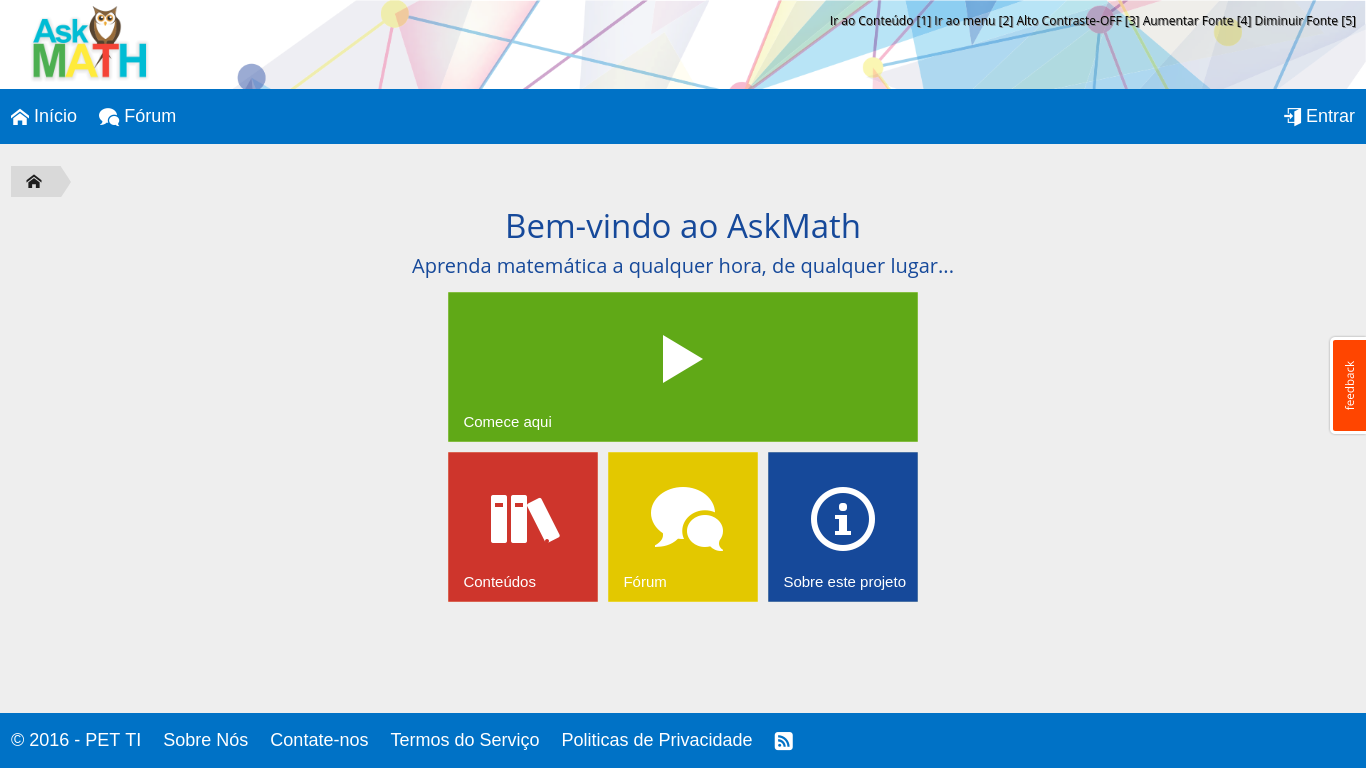
\includegraphics[width=\textwidth]{figuras/askmath/1}}
    }{
    \Fonte{\url{www.askmath.quixada.ufc.br}}
    }
  \end{minipage}
  \hfill
  \begin{minipage}[b]{0.49\textwidth}
	\Caption{Tela com as lições de Proposições}
	\UFCfig{}{    
    	\fbox{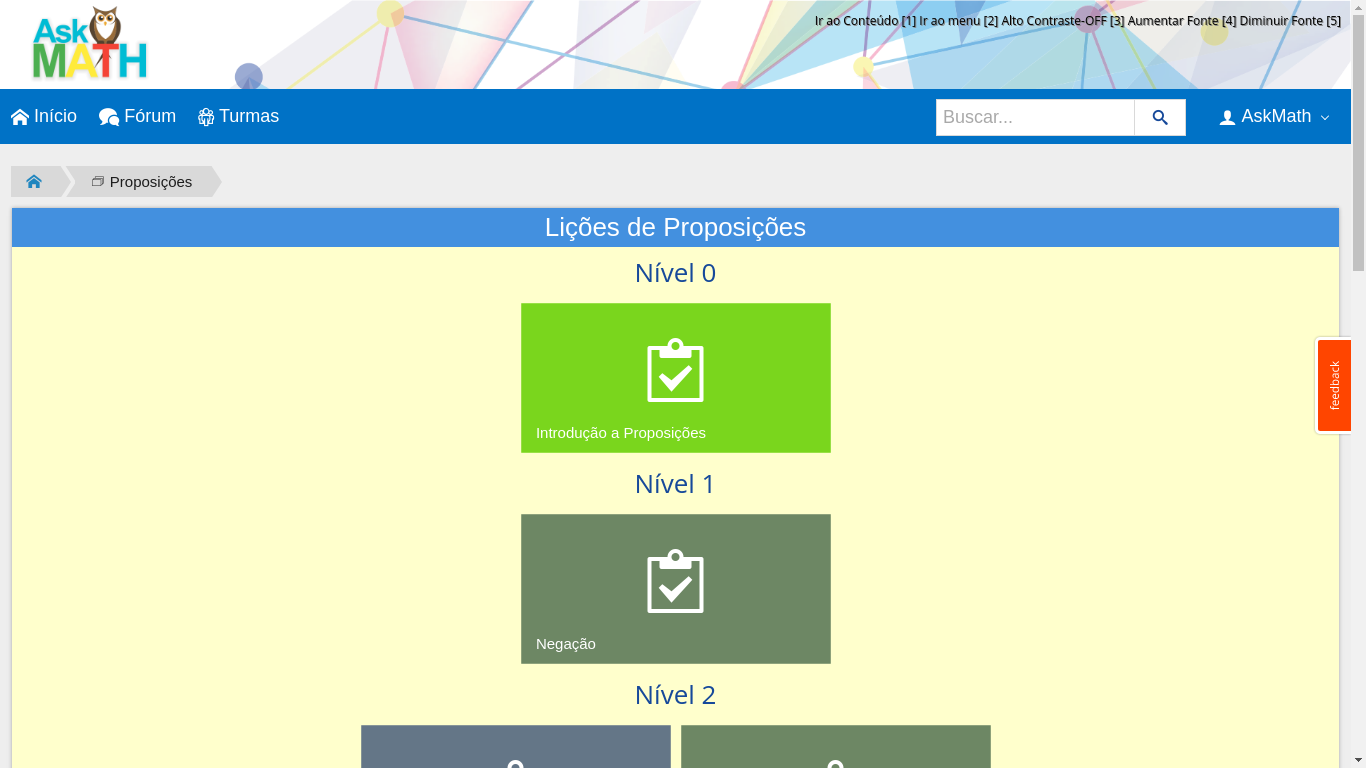
\includegraphics[width=\textwidth]{figuras/askmath/2}}
    }{
    \Fonte{\url{www.askmath.quixada.ufc.br}}
    }	
  \end{minipage}

\bigskip
 
  \begin{minipage}[b]{0.49\textwidth}
	\Caption{Tela de problemas do estudante}
	\UFCfig{}{    
    	\fbox{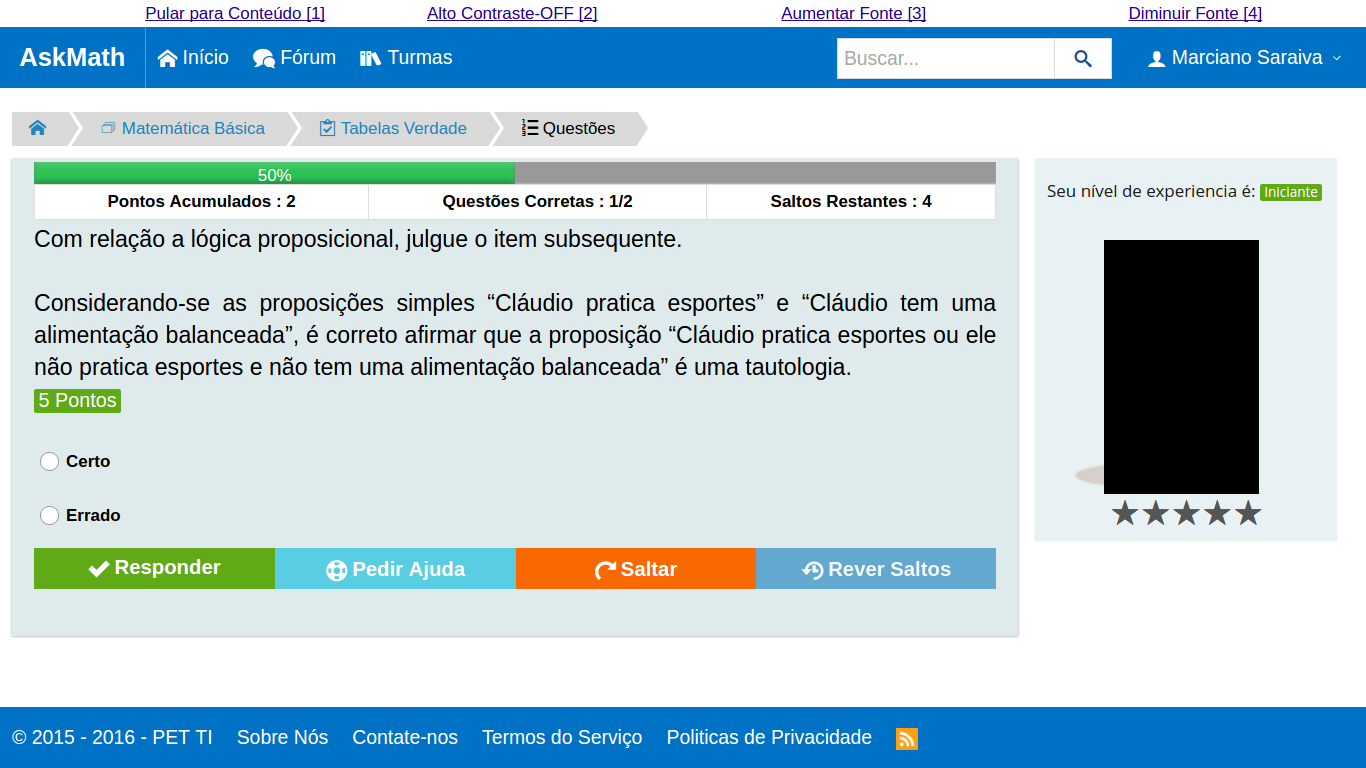
\includegraphics[width=\textwidth]{figuras/askmath/4}}
    }{
    \Fonte{\url{www.askmath.quixada.ufc.br}}
    }
  \end{minipage}
  \hfill
  \begin{minipage}[b]{0.49\textwidth}
	\Caption{Tela de uma postagem no fórum}
	\UFCfig{}{    
    	\fbox{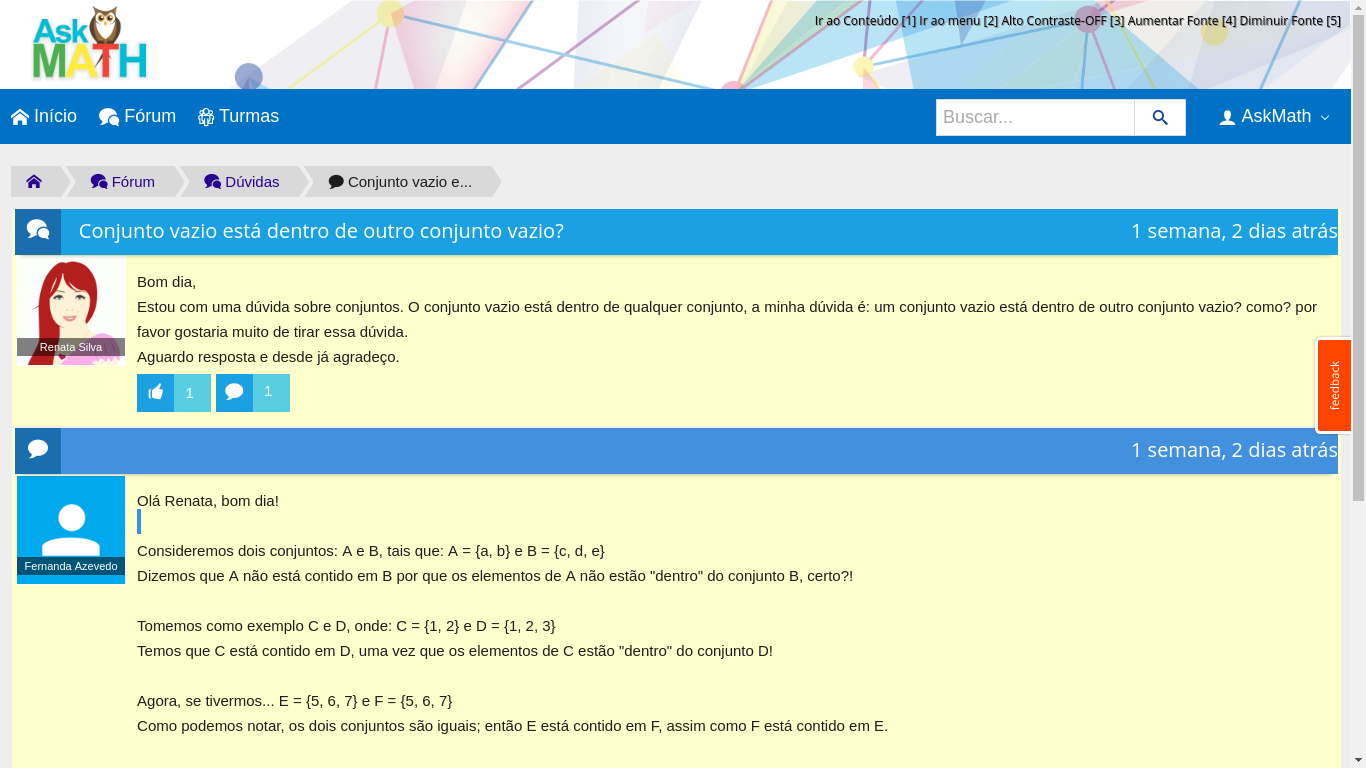
\includegraphics[width=\textwidth]{figuras/askmath/5}}
    }{
    \Fonte{\url{www.askmath.quixada.ufc.br}}
    }
  \end{minipage} 

\bigskip

   \begin{minipage}[b]{0.49\textwidth}
	\Caption{Tela de administra\c{c}\~ao}
	\UFCfig{}{    
    	\fbox{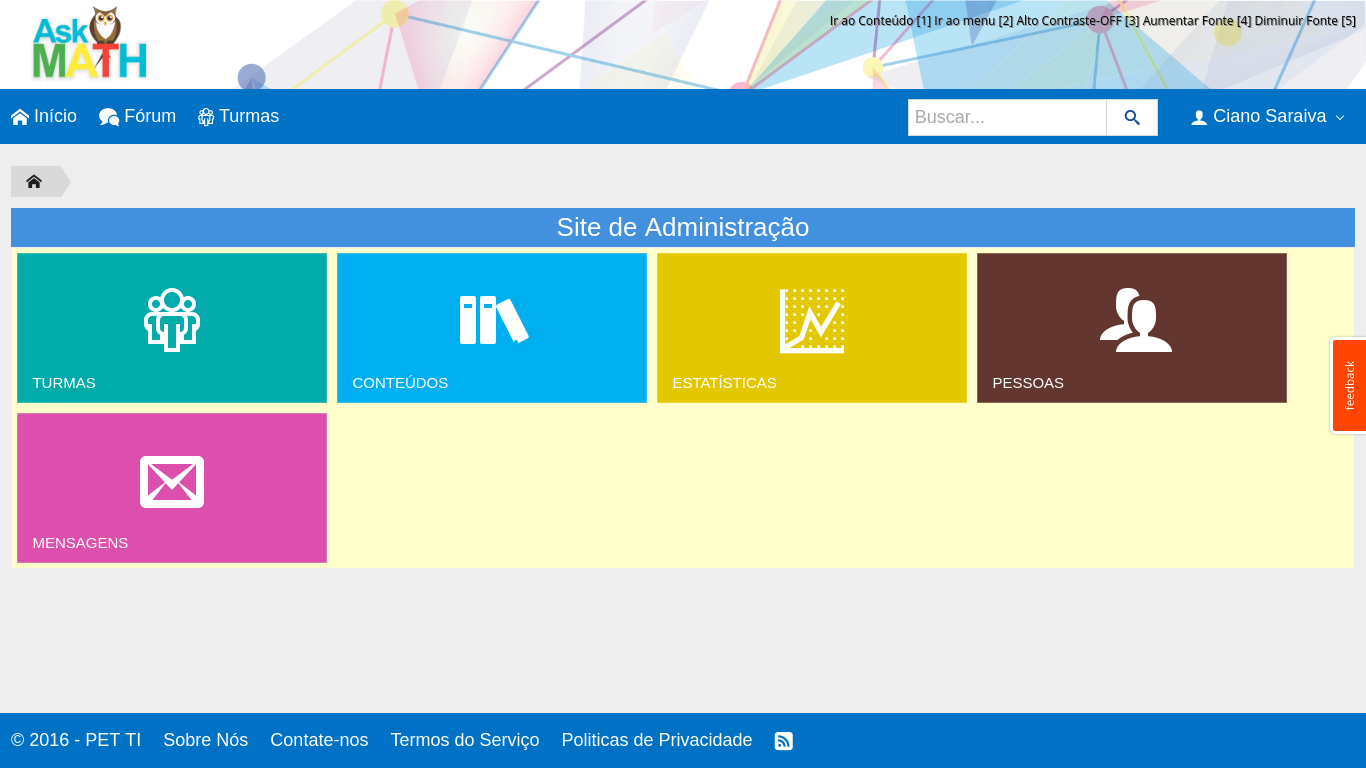
\includegraphics[width=\textwidth]{figuras/askmath/3}}
    }{
    \Fonte{\url{www.askmath.quixada.ufc.br}}
    }
  \end{minipage}
  \hfill
  \begin{minipage}[b]{0.49\textwidth}
	\Caption{Tela de problemas do administrador}
	\UFCfig{}{    
    	\fbox{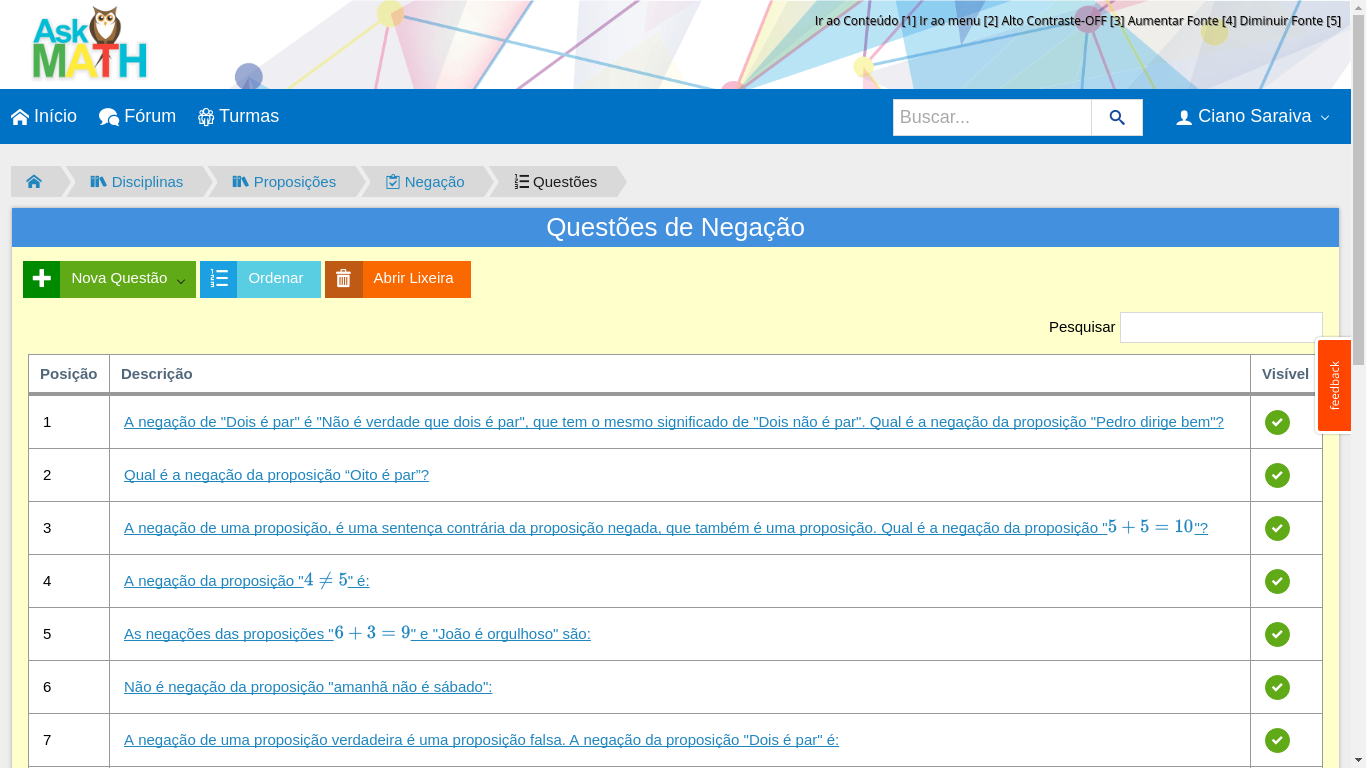
\includegraphics[width=\textwidth]{figuras/askmath/6}}
    }{
    \Fonte{\url{www.askmath.quixada.ufc.br}}
    }
  \end{minipage}  
\end{figure}

[FALAR DA AVALIAÇÂO AQUI]